\documentclass[conference]{IEEEtran}
\usepackage{graphicx} % Required for including images
\usepackage{amsmath} % Required for math environments
\usepackage{hyperref} % For hyperlinks
\usepackage{natbib} % For citations
\usepackage{float}
\usepackage{multirow}

% Citation aliasing
\defcitealias{IMDbDataset}{Maas et al., 2011}
\defcitealias{ApplicationsOfSA}{Pang and Lee, 2008}
\defcitealias{MLModelsUtility}{James et al., 2013}
\defcitealias{mikolov2013efficient}{Mikolov et al., 2013}

\begin{document}
	
	\title{Sentiment Analysis on IMDb Movie Reviews}
	\author{\IEEEauthorblockN{Aaron Pradhan}
		\IEEEauthorblockA{Khoury College of Computer Sciences\\
			Northeastern University\\
			Email: pradhan.aa@northeastern.edu}}
	\maketitle
	
	\begin{abstract}
		Sentiment analysis on movie reviews provides insights into consumer opinions, which are invaluable for producers, distributors, and content creators in the film industry. This paper outlines the application of machine learning models, namely Logistic Regression, Support Vector Machine (SVM), Random Forest, and Neural Networks, on the IMDb movie reviews dataset using pretrained Word2Vec embeddings to classify sentiments as positive or negative.
	\end{abstract}
	
	\IEEEpeerreviewmaketitle

	\section{Introduction}
	In the age of digital media, online movie reviews have become a crucial platform for gauging public opinion and sentiment towards cinematic productions. Analyzing these sentiments provides valuable insights for filmmakers, marketers, and audiences alike. Sentiment analysis, a key area within natural language processing (NLP), leverages computational techniques to identify and classify subjective information in text data. This study focuses on the sentiment analysis of movie reviews from IMDb, a rich repository of public opinion on films.
	
	The IMDb movie review dataset \citepalias{IMDbDataset} presents a unique challenge due to its unstructured and colloquial nature, requiring robust models capable of understanding complex linguistic nuances. To address this challenge, we employ four well-established machine learning models: Logistic Regression, Support Vector Machine (SVM), Random Forest, and Neural Networks. These models were chosen for their proven effectiveness in text classification tasks, with each bringing distinct advantages in terms of simplicity, flexibility, and robustness against overfitting. Machine learning models have been widely adopted due to their ability to learn from data and make predictions or decisions without being explicitly programmed to perform the task \citep{MLModelsUtility}.

	A critical aspect of our approach is the utilization of Word2Vec embeddings \citepalias{mikolov2013efficient}. Originally developed by researchers at Google, Word2Vec provides a powerful method for transforming words into meaningful numerical representations, capturing semantic and syntactic relationships in a high-dimensional space. By leveraging the pretrained Word2Vec embeddings based on the Google News dataset, we aim to enrich our models' capabilities in discerning sentiment, allowing for a more nuanced and accurate classification of movie reviews.

	Through this research, we aim to not only contribute to the understanding of sentiment analysis in the context of movie reviews but also to demonstrate the practical application and effectiveness of machine learning models when combined with advanced word embeddings. The findings of this study have the potential to inform content creators and distributors in the film industry, offering a data-driven perspective on audience reception and preferences. Additionally, understanding movie review sentiments can guide movie recommendations and forecast box office success \citepalias{ApplicationsOfSA}.
	
	\section{Data}
	
	The dataset used for this study is the IMDb movie review dataset, which is a popular benchmark dataset in natural language processing and sentiment analysis research. It consists of 50,000 movie reviews from the IMDb website, with labels indicating the sentiment of the review. The dataset is evenly split into 25,000 reviews for training and 25,000 for testing, ensuring that there is no overlap in movies between the training and test sets. Each set contains an equal number of positive and negative reviews, where a positive review has a rating of 7 or higher out of 10, and a negative review has a rating of 4 or lower. Reviews with more neutral ratings are not included in the dataset.

	Prior to modeling, the reviews underwent several preprocessing steps. First, HTML tags were removed, and the text was converted to lowercase. Special characters were stripped, and the text was tokenized into individual words. Stop words were filtered out to reduce noise in the data, and words were lemmatized to their base forms.

	For the Logistic Regression, Support Vector Machine, and Random Forest models, the words were transformed into numerical features using the pretrained Word2Vec Google News 300 Embeddings. For the Neural Network, each word was represented by an integer index. To address the variable length of reviews as inputs to the Neural Network, the sequences were padded to a uniform length, with excessively long reviews truncated and shorter ones padded with zeros. This preprocessing resulted in a consistent and structured input format suitable for training the sentiment analysis models.

	\section{Implementation}
	
	\subsection{Logistic Regression}
	
	Logistic Regression is a statistical model that in its basic form uses a logistic function to model a binary dependent variable. In the context of sentiment analysis, logistic regression was applied as a baseline classifier. Given the high dimensionality of the input data after text preprocessing, logistic regression can perform well as it is less prone to overfitting. The implementation of the logistic regression classifier was done using the \texttt{LogisticRegression} class from the scikit-learn library.
	
	\subsection{Support Vector Machine}
	
	The Support Vector Machine (SVM) classifier is a powerful and versatile machine learning model, capable of performing linear or non-linear classification. For this project, the SVM was implemented using the \texttt{SVC} class from the scikit-learn library, with a radial basis function (RBF) kernel to handle the non-linearity in the dataset.
	
	The training process involved mapping the review data into a higher dimensional space where a hyperplane could be found that best separates the data into positive and negative sentiment classes. Key hyperparameters for the SVM, including the penalty parameter $C$ and the kernel coefficient $\gamma$, were optimized using a grid search approach with cross-validation. A range of values for $C$ and $\gamma$ were evaluated to identify the combination that maximized the margin between classes while minimizing classification error.
	
	The final SVM model, with optimized hyperparameters, provided a non-linear decision boundary that could effectively handle the complexities inherent in natural language data. The performance of the SVM was expected to surpass the logistic regression baseline due to its ability to capture the high-dimensional patterns present in the text data.
	
	\subsection{Random Forest}
	
	The Random Forest classifier was initially employed using its default parameters as provided by the \texttt{RandomForestClassifier} in the scikit-learn library. This served as a baseline from which to understand the model's performance without hyperparameter tuning. Despite its robustness and capability to handle nonlinear relationships, the baseline model did not achieve performance on par with Logistic Regression or SVM.
	
	To optimize the Random Forest, a hyperparameter search was conducted using \texttt{GridSearchCV}, with a focus on parameters believed to be most influential based on the literature and default settings. A preliminary test was performed to determine if training on a subset of the data would yield comparable accuracies to using the full dataset. This was motivated by the desire to reduce computational costs during grid search. It was found that training on 20\% of the data resulted in an accuracy that was only 0.005 less than the model trained on the entire dataset, which was deemed an acceptable trade-off for the increased efficiency.
	
	The selected parameters for the grid search were as follows:
	
	\begin{verbatim}
		rf_param_grid = {
			'n_estimators': [100, 200],
			'max_depth': [None, 10, 20],
			'min_samples_split': [2, 10],
			'min_samples_leaf': [1, 5],
			'bootstrap': [True],
			'criterion': ['gini']
		}
	\end{verbatim}
	
	The grid search revealed that variations in the \texttt{max\_depth} parameter had minimal impact on the model's accuracy. Consequently, a second grid search was performed with a refined parameter space, particularly focusing on \texttt{n\_estimators}, \texttt{min\_samples\_split}, and \texttt{min\_samples\_leaf} around their previously determined optimal values. Despite these efforts, the highest mean cross-validated accuracy obtained was below 0.82, prompting the decision to discontinue further exploration of the Random Forest model.
	
	\subsection{Neural Network}
	
	In contrast to the traditional machine learning approaches, the Neural Network was designed to capture the sequential nature of text data. The architecture was built using Keras, with a tokenization process that represented words as integers, capturing the top 40,000 words to include the vast majority of the vocabulary present in the reviews. This was followed by sequence padding to a fixed length of 250 words, which accommodated the majority of the review lengths.
	
	The network started with an embedding layer designed for a 40,000-word vocabulary, outputting 32-dimensional embeddings. This was followed by a flattening layer, transforming the 2D embedding output to 1D for processing in subsequent dense layers. The choice to flatten the embeddings was made to simplify the model architecture. The flattened layer was followed by a dense layer with 256 units, which included L2 regularization to address overfitting observed in earlier epochs. A dropout layer with a rate of 0.6 further aided in regularization. The output layer consisted of a single neuron with a sigmoid activation function, reflecting the binary nature of the sentiment classification task. The Adam optimizer was selected for its adaptive learning rate capabilities, and binary cross-entropy was used as the loss function due to its suitability for binary classification problems.
	
	After initial overfitting, early stopping with a patience of 3 epochs was introduced, and the number of units in the dense layer was reduced. Additionally, the learning rate was decreased to encourage more stable and gradual learning. The final model was subjected to a 5-fold cross-validation, achieving a mean accuracy of 0.881, with a low standard deviation, indicating both high performance and model stability.
	
	The final iteration of the neural network was trained on the full training set and tested on the separate test set, where it achieved an accuracy of 0.8622, validating the effectiveness of the neural network approach for this sentiment analysis task.
	
	\section{Results}
	
	\subsection{Support Vector Machine}
	The Support Vector Machine (SVM) models, with their capacity for high-dimensional data, were fine-tuned through grid search, optimizing the $C$ and $\gamma$ parameters. Two heatmaps were generated to visualize the performance landscape over the parameter grid.
	
	\begin{figure}[htbp]
		\centering
		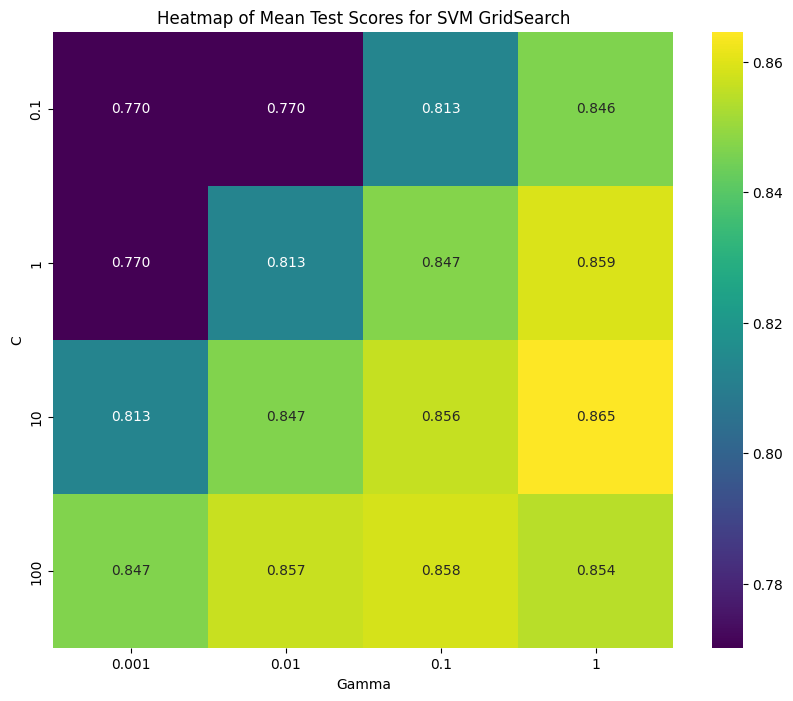
\includegraphics[width=0.5\textwidth]{svm_heatmap1.png}
		\caption{Heatmap of the first SVM grid search results showing the cross-validation accuracy for combinations of $C$ and $\gamma$.}
		\label{fig:svm_heatmap1}
	\end{figure}
	
	\begin{figure}[htbp]
		\centering
		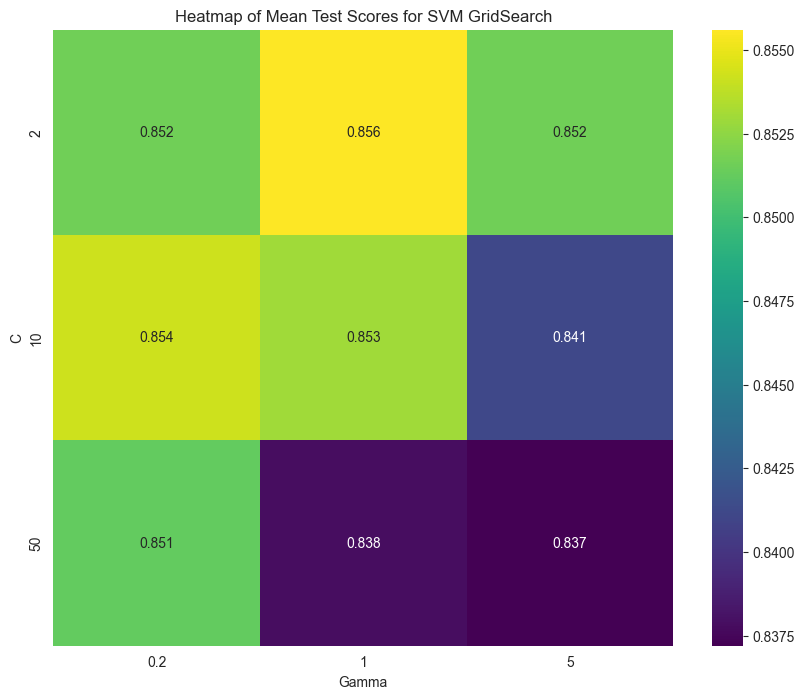
\includegraphics[width=0.5\textwidth]{svm_heatmap2.png}
		\caption{Heatmap of the second, focused SVM grid search results.}
		\label{fig:svm_heatmap2}
	\end{figure}
	
	The heatmaps (\ref{fig:svm_heatmap1}) and (\ref{fig:svm_heatmap2}) illustrate the sensitivity of the model accuracy to the hyperparameters, guiding the selection of the final model parameters.
	
	\subsection{Random Forest}
	The baseline Random Forest model's performance increased marginally when the training data was scaled up incrementally. A plot of model accuracy versus the percentage of the training data used highlighted the diminishing returns on accuracy with increased data usage.
	
	\begin{figure}[htbp]
		\centering
		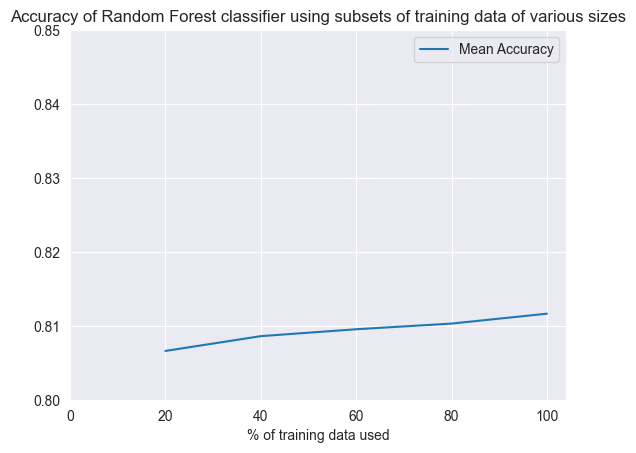
\includegraphics[width=0.5\textwidth]{rf_accuracy_plot.png}
		\caption{Accuracy of the Random Forest classifier against different subsets of the training data.}
		\label{fig:rf_accuracy_plot}
	\end{figure}
	
	Subsequent grid searches provided insights into the effect of various hyperparameters, visualized through bar plots.
	
	\begin{figure}[htbp]
		\centering
		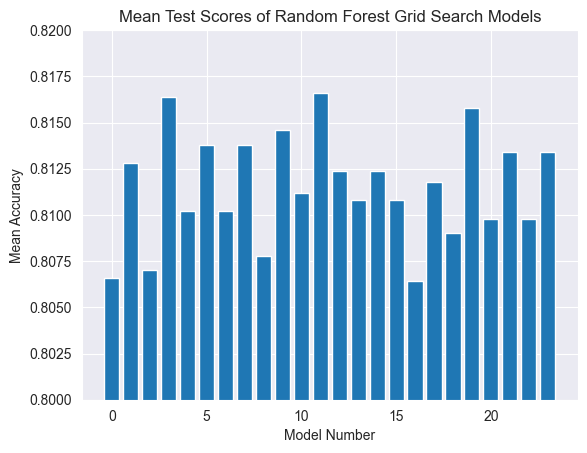
\includegraphics[width=0.5\textwidth]{rf_barplot1.png}
		\caption{Bar plot from the first Random Forest grid search.}
		\label{fig:rf_barplot1}
	\end{figure}
	
	\begin{figure}[htbp]
		\centering
		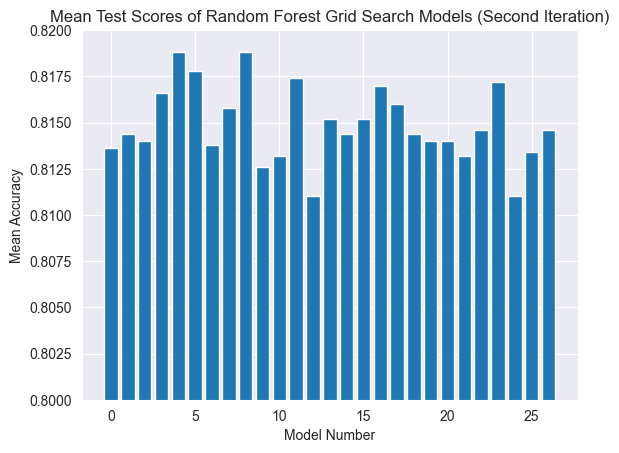
\includegraphics[width=0.5\textwidth]{rf_barplot2.png}
		\caption{Bar plot from the refined Random Forest grid search.}
		\label{fig:rf_barplot2}
	\end{figure}
	
	Although the hyperparameter tuning (\ref{fig:rf_barplot1}) and (\ref{fig:rf_barplot2}) offered improvements, the Random Forest classifier did not achieve an accuracy that warranted further consideration as a final model.
	
	\subsection{Neural Network}
	The distribution of review lengths was captured in a histogram, which informed the decision to pad sequences to a length of 250 words.
	
	\begin{figure}[htbp]
		\centering
		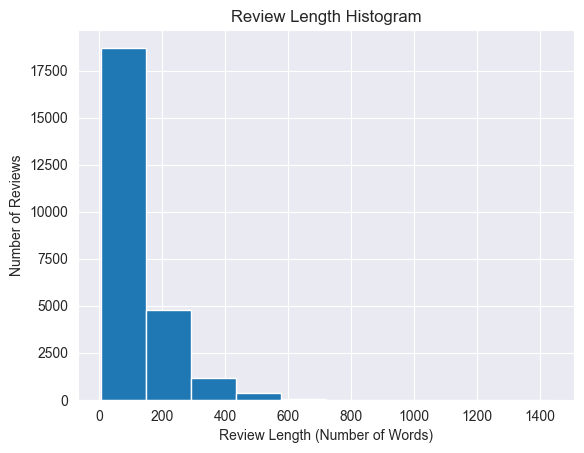
\includegraphics[width=0.5\textwidth]{review_length_histogram.png}
		\caption{Histogram of the review length distribution in the training dataset.}
		\label{fig:review_length_histogram}
	\end{figure}
	
	Two iterations of neural network training were conducted, with the training and validation loss for each plotted to illustrate the learning process and the effect of implemented regularizations.
	
	\begin{figure}[htbp]
		\centering
		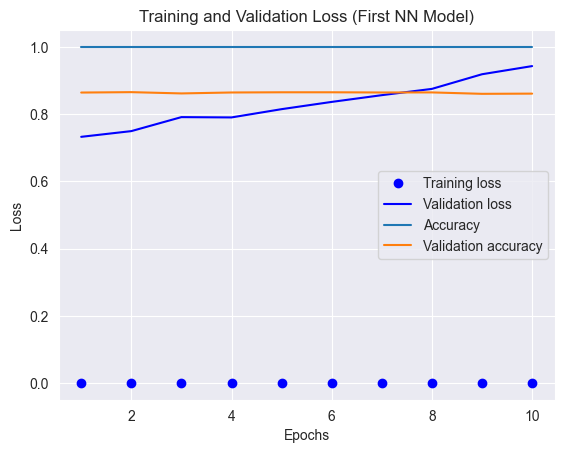
\includegraphics[width=0.5\textwidth]{nn_loss_plot1.png}
		\caption{Training and validation loss from the initial neural network model.}
		\label{fig:nn_loss_plot1}
	\end{figure}
	
	\begin{figure}[htbp]
		\centering
		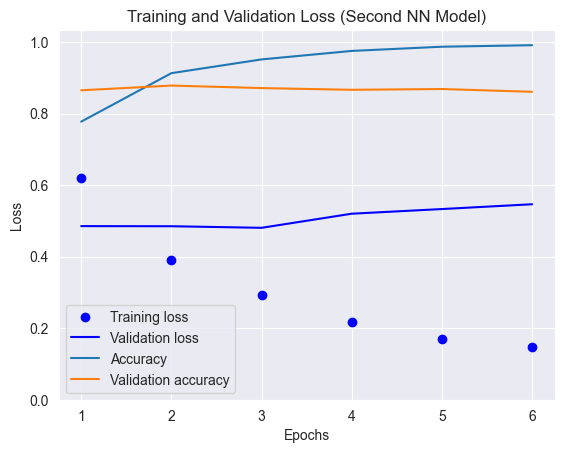
\includegraphics[width=0.5\textwidth]{nn_loss_plot2.png}
		\caption{Training and validation loss after applying early stopping and regularization.}
		\label{fig:nn_loss_plot2}
	\end{figure}
	
	The final neural network model demonstrated a balanced classification performance, as reflected in the classification report and the confusion matrix.
	
	\begin{table}[htbp]
		\centering
		\begin{tabular}{lcccc}
			\hline
			Class & Precision & Recall & F1-Score & Support \\ \hline
			0     & 0.86      & 0.87   & 0.86     & 12500   \\
			1     & 0.87      & 0.86   & 0.86     & 12500   \\ \hline
		\end{tabular}
		\caption{Classification report for the final neural network model.}
		\label{tab:classification_report}
	\end{table}
	
	\begin{table}[htbp]
		\centering
		\caption{Confusion Matrix for the final neural network model.}
		\label{tab:confusion_matrix}
		\begin{tabular}{cc|cc}
			\multicolumn{2}{c}{} & \multicolumn{2}{c}{Predicted} \\
			& & 0 & 1 \\ 
			\cline{2-4}
			\multirow{2}{*}{\rotatebox[origin=c]{90}{Actual}}
			& 0 & 10865 & 1635 \\
			& 1 & 1810 & 10690 \\
		\end{tabular}
	\end{table}
	
	\section{Conclusion}
	
	This study presented a comprehensive analysis of sentiment classification on the IMDb movie review dataset. We explored a variety of machine learning models, including Logistic Regression, Support Vector Machines, Random Forest, and Neural Networks, each offering unique insights into the sentiment analysis task.
	
	Logistic Regression served as a solid baseline, providing a benchmark for model performance with its simplicity and interpretability. Support Vector Machines demonstrated a notable improvement in accuracy, capitalizing on their ability to handle high-dimensional spaces and intricate data distributions.
	
	Our experiments with Random Forest classifiers, although insightful, revealed limitations in handling the nuances of textual data as compared to the other models. Despite hyperparameter tuning efforts, the performance of Random Forest classifiers did not surpass that of SVM or Neural Networks.
	
	The Neural Network, with its deep learning capabilities, outperformed the traditional machine learning models. The utilization of Word2Vec embeddings to capture semantic and syntactic word relationships significantly contributed to the model's performance. By leveraging these embeddings, we were able to train a model that not only recognized the sentiment of movie reviews with high accuracy but also proved to be robust against overfitting, thanks to carefully implemented regularization techniques and early stopping.
	
	Future work may involve experimenting with more complex deep learning architectures, such as recurrent neural networks or transformers, which could potentially capture the sequential nature of language even more effectively. Additionally, exploring other word embeddings or fine-tuning on domain-specific corpora could further enhance model performance.
	
	In conclusion, our study underscores the effectiveness of neural networks in sentiment analysis and highlights the importance of thoughtful preprocessing and model selection in natural language processing tasks. The advancements in word embeddings and deep learning continue to push the boundaries of what is possible in the field of sentiment analysis.
	
	\bibliographystyle{IEEEtran}
	\bibliography{references}
	
\end{document}
